\appendix
\addappheadtotoc
\counterwithin{figure}{section}
\section{Appendix}
\label{sec:sec010}

%%%%%%%%%%%%%%%%%%%%%%%%%%%%%%%%%%%%%%%%%%%%%%%%%%%
\begin{figure}[htbp]
\onecolumn
\centering
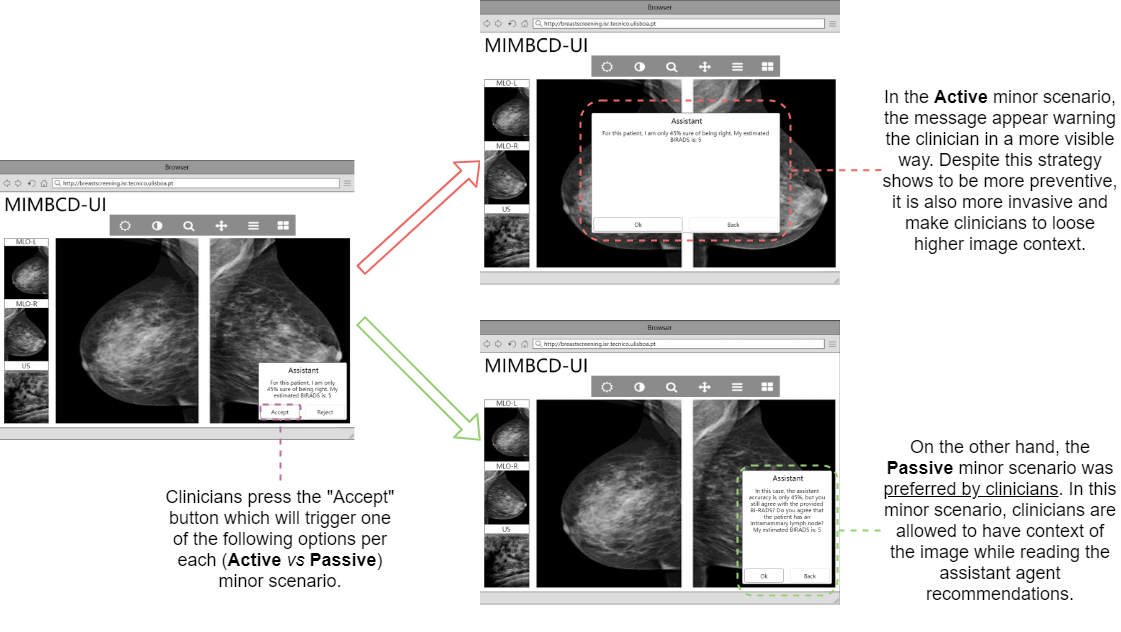
\includegraphics[width=0.95\textwidth]{fig022}
\caption{When the clinician press the "Accept" button, the system will trigger two minor scenario options: (a) {\bf Active}; or (b) {\bf Passive}. During our sessions of low-fi prototype co-design with clinicians, all of them preferred the (b) {\bf Passive} option.}
\label{fig:fig022}
\twocolumn
\end{figure}
%%%%%%%%%%%%%%%%%%%%%%%%%%%%%%%%%%%%%%%%%%%%%%%%%%%

%%%%%%%%%%%%%%%%%%%%%%%%%%%%%%%%%%%%%%%%%%%%%%%%%%%
\begin{figure}[htbp]
\onecolumn
\centering
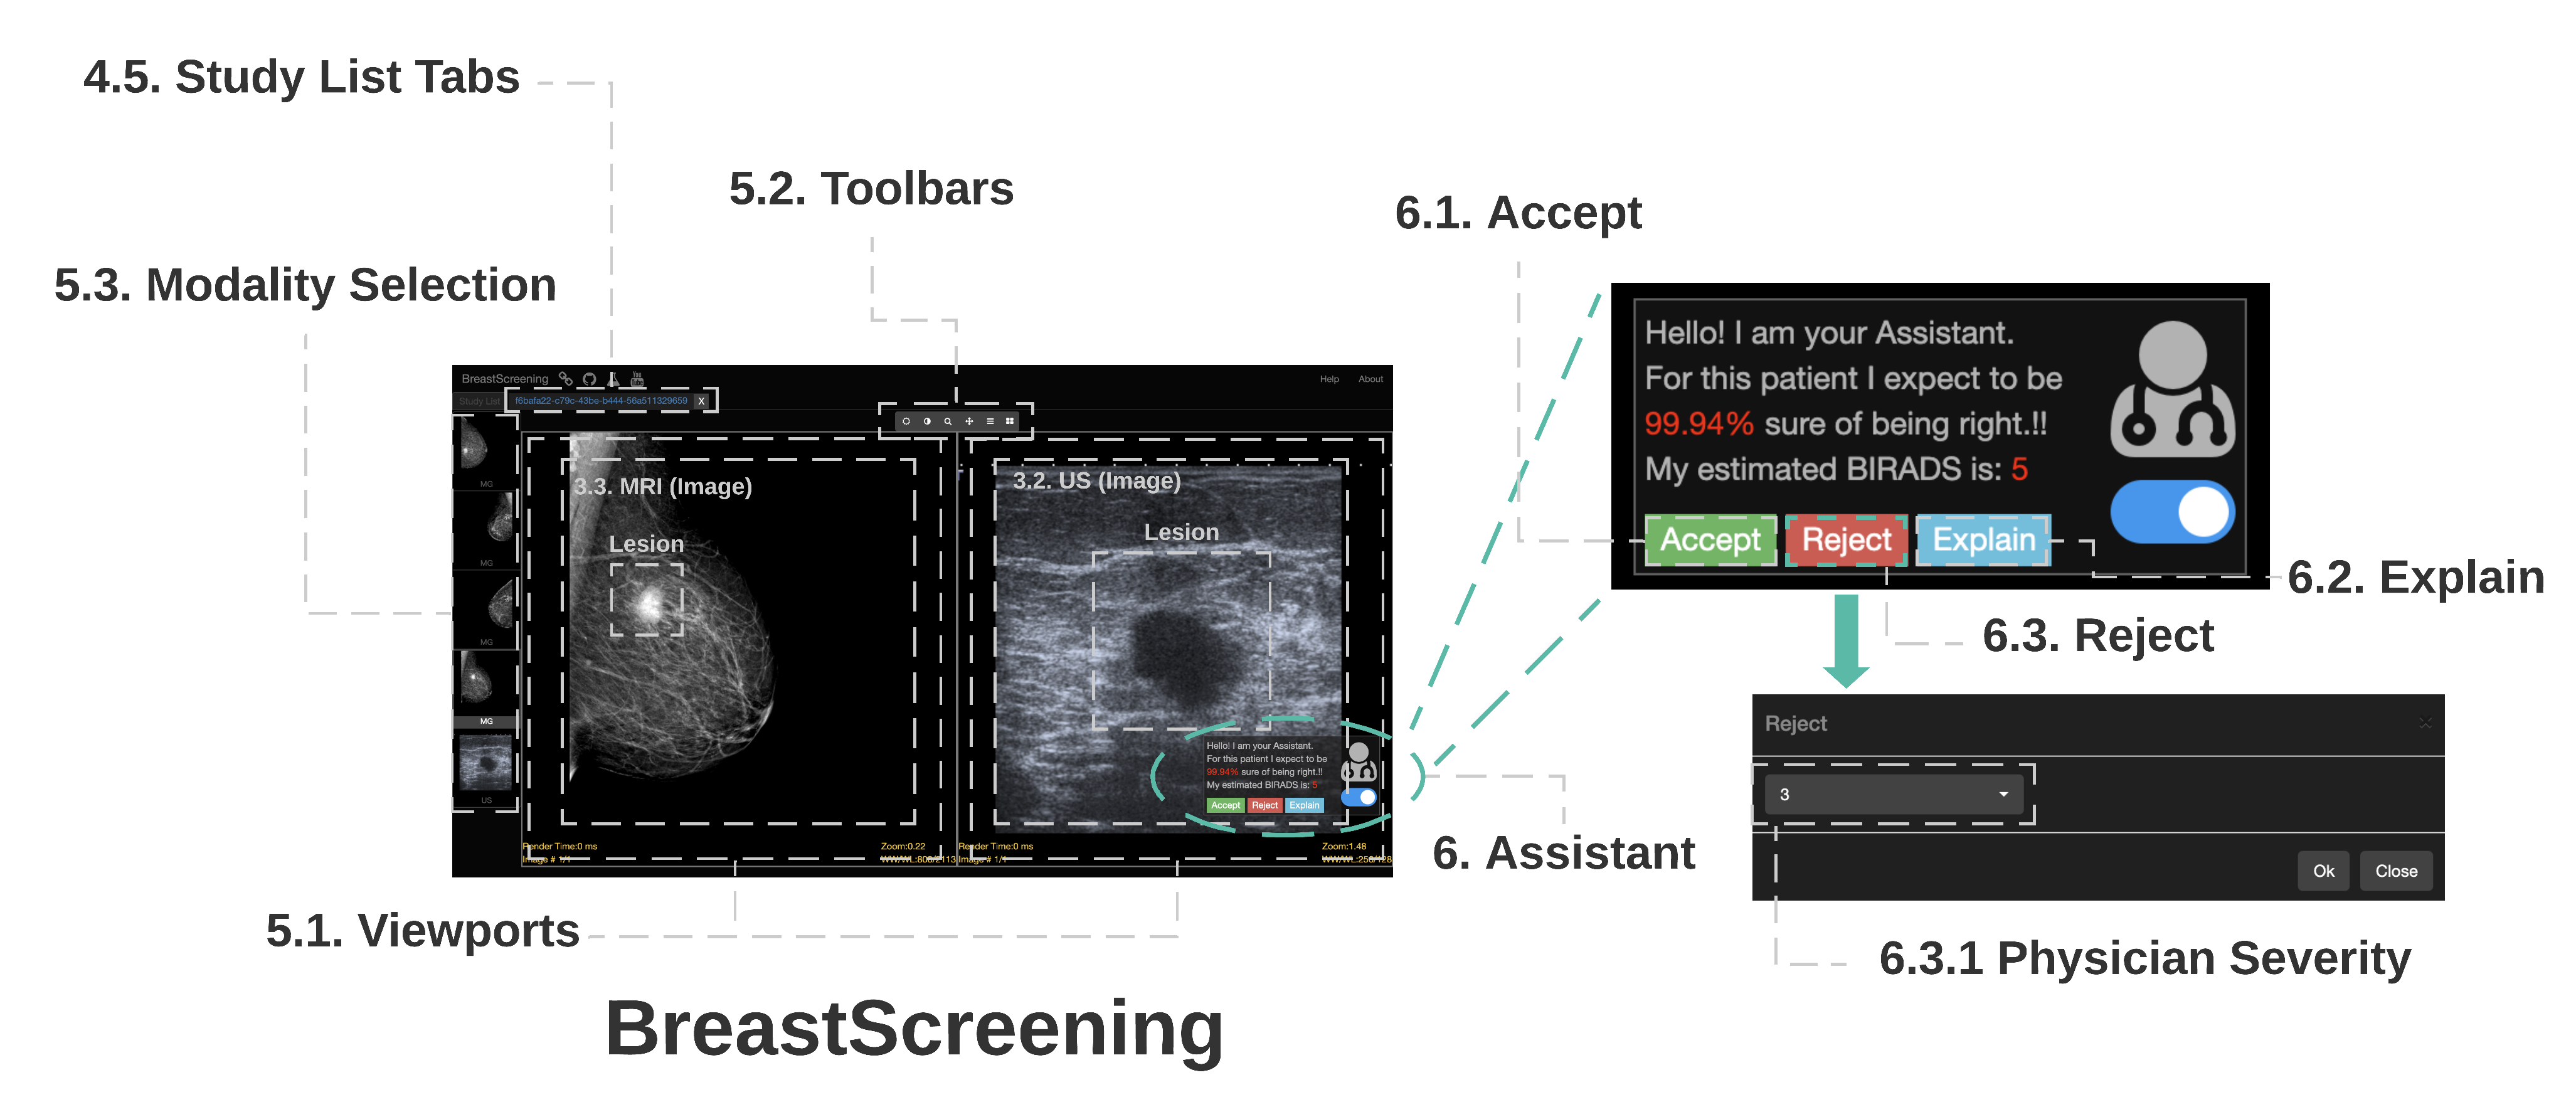
\includegraphics[width=0.95\textwidth]{fig002}
\caption{Our {\it BreastScreening} assistant provides several features regarding the basics of medical imaging diagnostic. From there, we will be able to validate our DenseNet BIRADS classifier along with clinicians.}
\label{fig:fig002}
\twocolumn
\end{figure}
%%%%%%%%%%%%%%%%%%%%%%%%%%%%%%%%%%%%%%%%%%%%%%%%%%%

\clearpage

%%%%%%%%%%%%%%%%%%%%%%%%%%%%%%%%%%%%%%%%%%%%%%%%%%%
\begin{figure}[t!]
\onecolumn
\centering
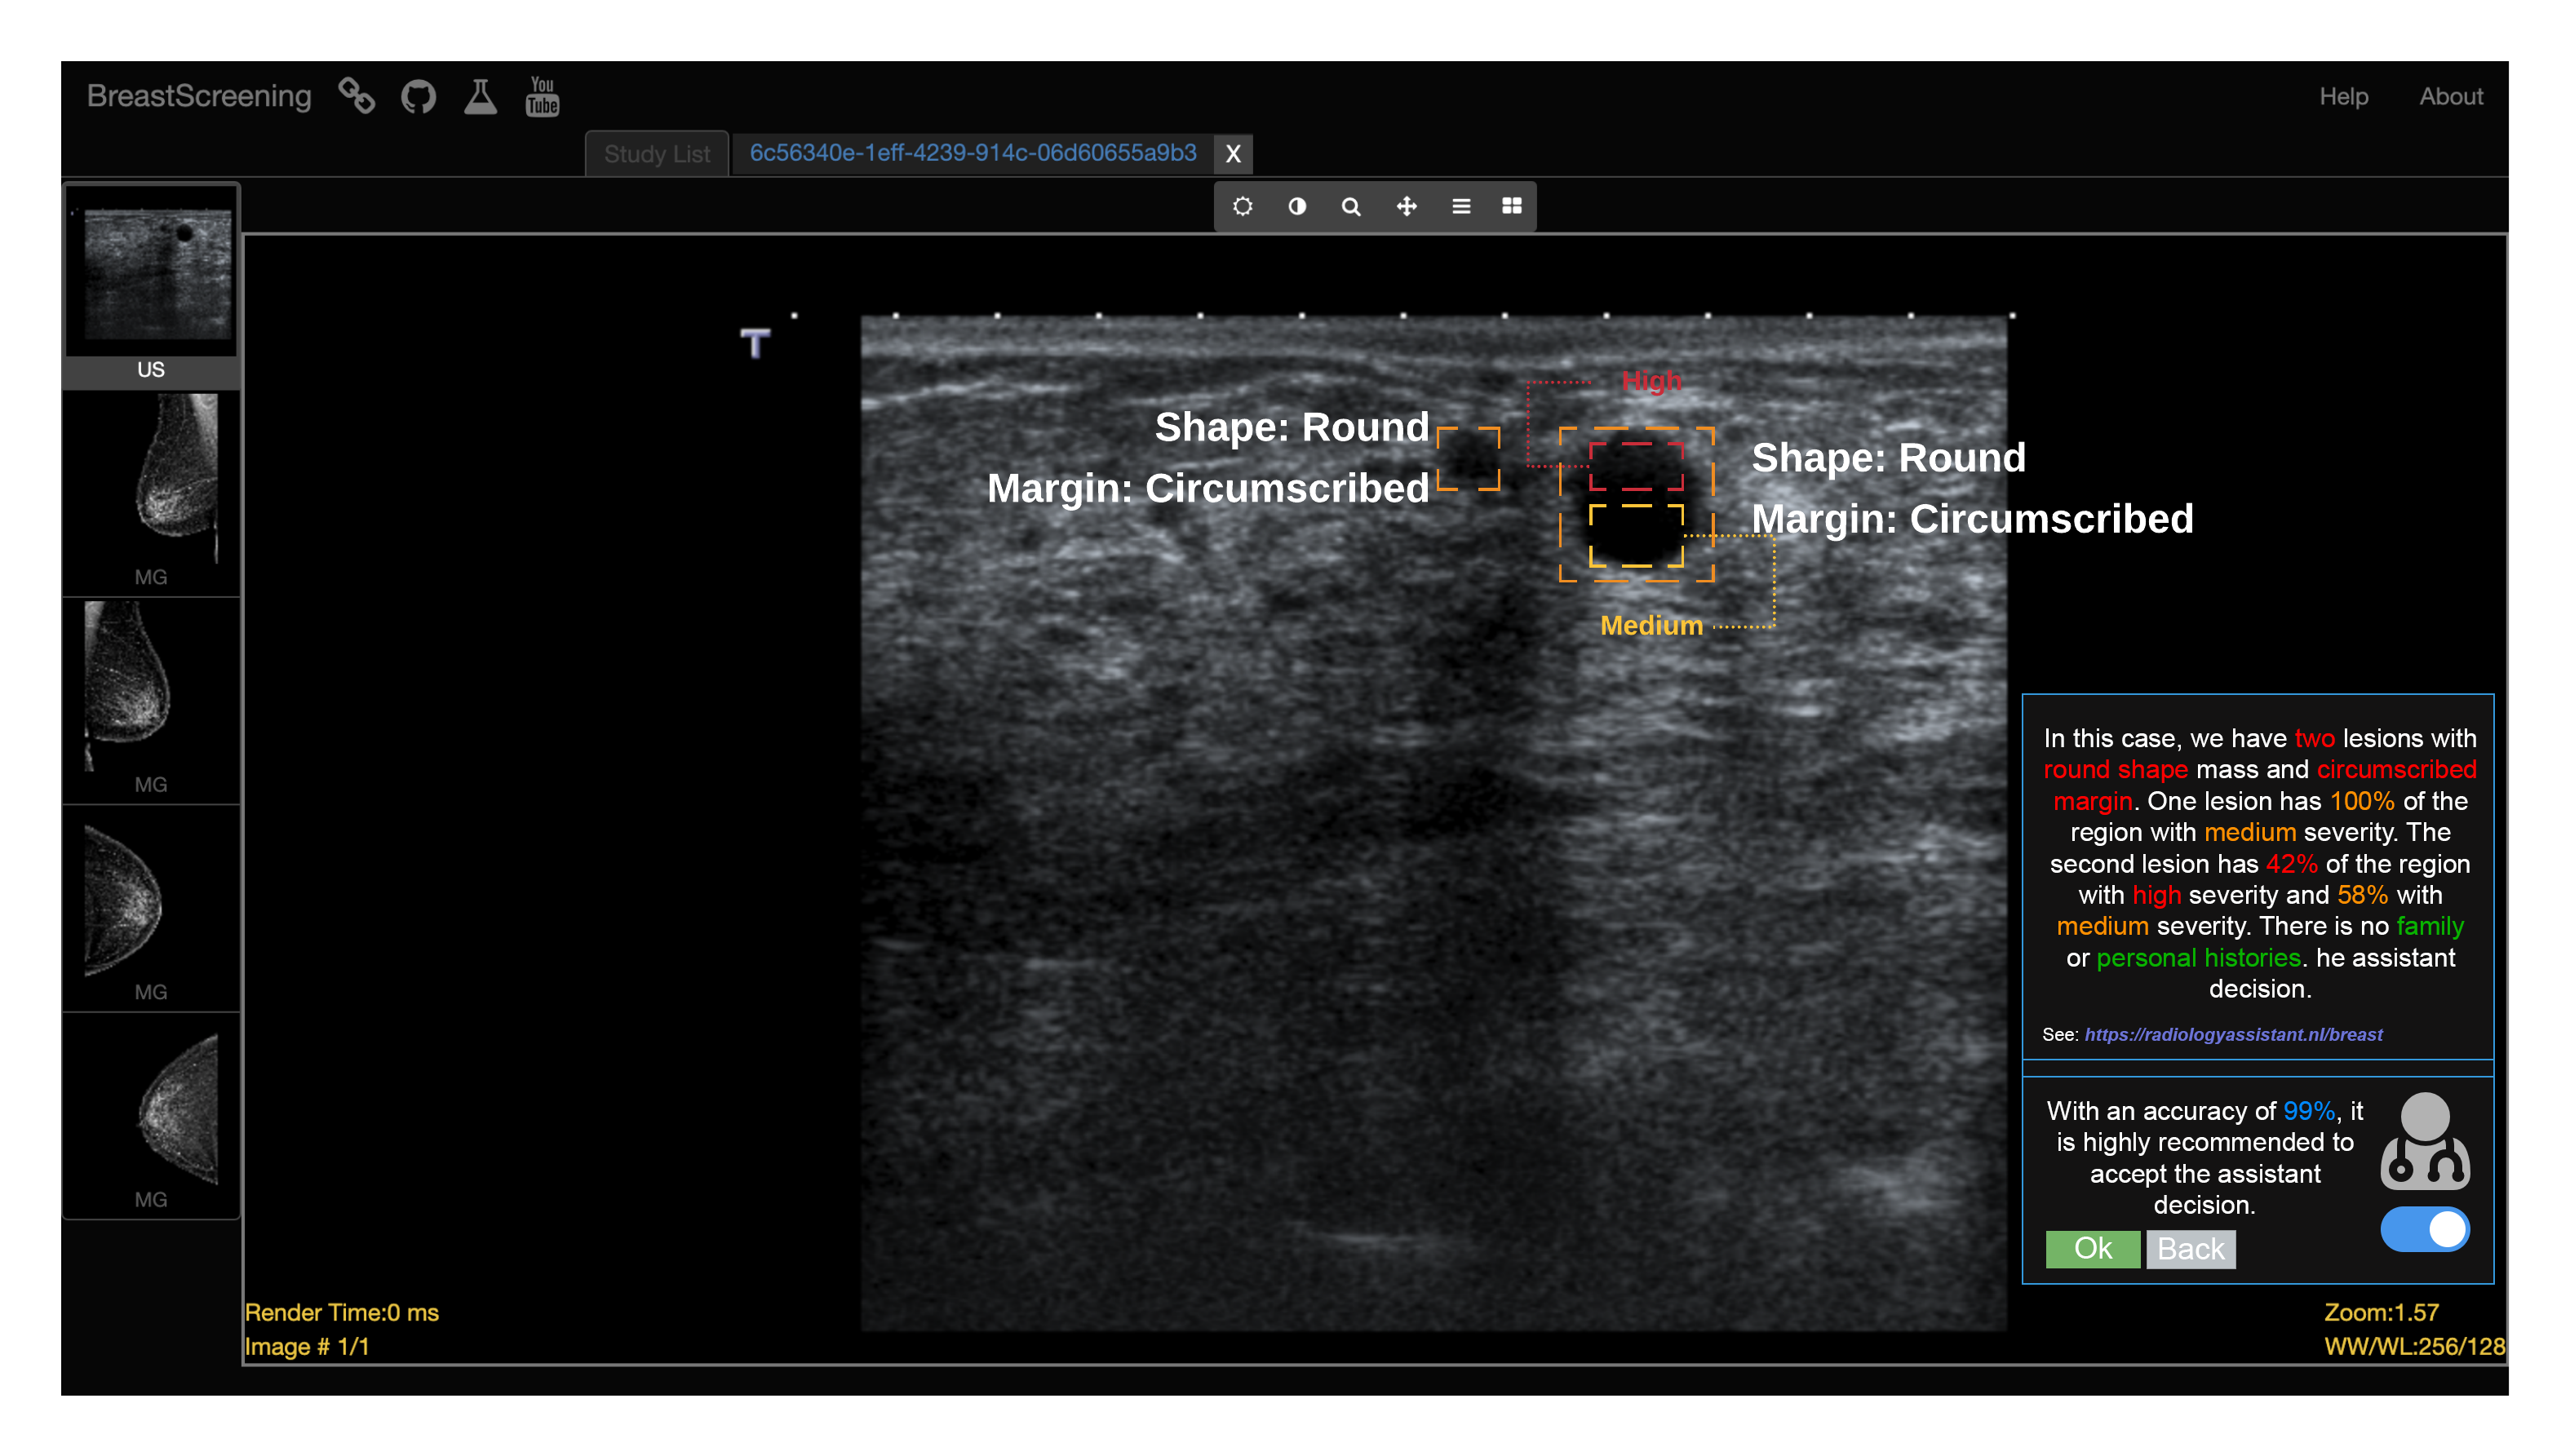
\includegraphics[width=\textwidth]{fig024}
\caption{Here, we propose the suggested system resulted from a preliminary evaluation. From this proposed system, we will be able to understand when ({\it e.g.}, {\bf Proactive} {\it vs} {\bf Reactive}) and how ({\it e.g.}, {\bf Assertive} {\it vs} {\bf Non-Assertive}) should the assistant agent adapt and change the behaviour per each group ({\it i.e.}, Interns, Juniors, Middles and Seniors) of medical experience. In this case, we have an {\bf Assertive} communication with the second screen of a {\bf Reactive} agent.}
\label{fig:fig024}
\twocolumn
\end{figure}
%%%%%%%%%%%%%%%%%%%%%%%%%%%%%%%%%%%%%%%%%%%%%%%%%%%